\chapter{Prospects for Neutral MSSM Higgs Search Improvement}

The neutral MSSM Higgs search, described in the previous chapter, 
suffers strongly of poor jet reconstruction efficiency and  b-tagging performance due to the particular phase space
required, this bound the potential of this search, improoving b-tagging
would result in a major improvement of the search sensitivity. 
This chapter investigates an alternative to the commonly used calorimeter jets in ATLAS, 
which is trackjets b-tagging. 
The prospects for successfully use trackjets b-tagging in the future neutral MSSM Higgs searches are reported,
b-tagging on trackjets was never attempted before.
Section\ref{bla} describes this and that...


\clearpage

\section{Introduction to Trackjets} \label{sec:tj_intro}
% reasonable intro + ++ 
This problematic has two sources:
- The ATLAS calorimeter is not a sampling calorimeter, this means that responses differently 
for Hadrons and for leptons, has different responses to electromagnetic and hadronic shower.
The Calorimeter cells are calibrated in energy using response to electromagnetic showers, to 
know the energy of the original parton that initiated the jet there are different procedure 
to calibrate the Jets offline which are called in short Jet Energy Scale (JES) corrections \cite{}, 
which make use of MC simulation.
Due to the high amount of pileup and ambient energy density in the events, jets are calibrated % also other problems: underlying event ecc..
from 20 GeV in $\pt$, this means that currently is not possible with calorimeter jets to access the
low transverse momentum phase space.

\begin{figure}[tp]
     \begin{center}

            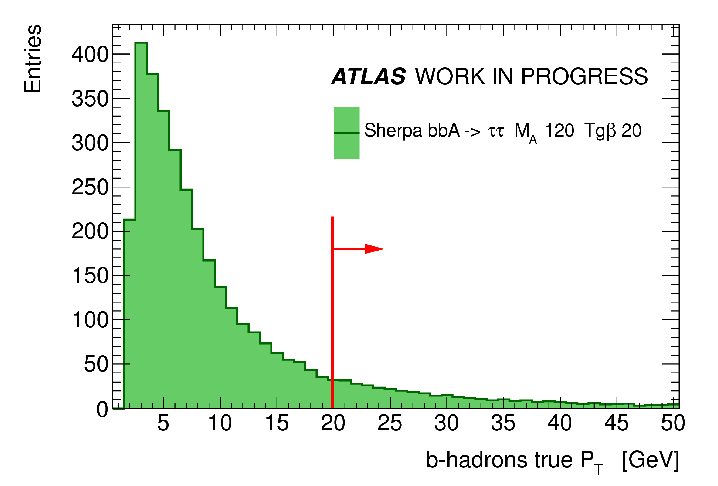
\includegraphics[width=0.49\textwidth]{figure/trackjet/bbA_pt.png}
            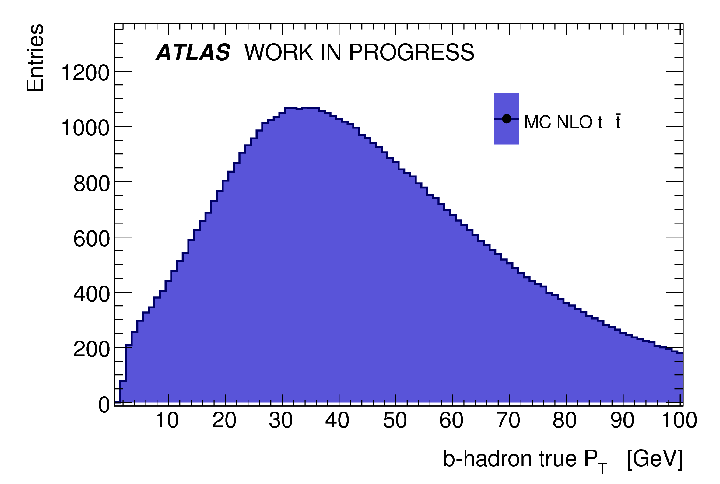
\includegraphics[width=0.49\textwidth]{figure/trackjet/top_pt.png}

    \end{center}
    \caption{Cormparison of simulated b-hadron distribution for signal b-associated production events (left) and $\ttbar$ events (right).
	The red line in the figure shows the acceptance region due to calibrated jet $\pt$ requirements.}
   \label{fig:bjetDistro}
\end{figure}

The neutral MSSM Higgs search, as described in chapter~\ref{chap:anal}, splits the dataset in two category
by means of the presence or the absence of a b-tagged jet, the b-tagged category is optimized for the b-associated production 
mechanism, in which the Higgs is produced in association with two b-jets. Figure~\ref{fig:bjetDistro} shows a comparison 
between $\pt$ spectrum of simulated b-hadron in b-associated Higgs  and $\ttbar$ events, the signal prefers b-hadron with 
relatively low transverse momentum,  jet calibration invoqe jet $\pt > 20$ GeV removing a large fraction of possible
signal candidate, many of the b-associated production signal events falls in fact in the b-veto category, making 
the separation not so effective.
The low $\pt$ spectrum is actually quite challenging, jet reconstruction efficiency and calibration set then a lower limit
to the signal sensitivity in the b-tag category.
Another challenge to this search are the poor b-tagging performance at low transverse momentum, for the a fixed tagging point of the 
MV1 tagger the b-tagging efficiency drops, in fact,  rapidly  with jet $\pt$ reacing a minimum of 50\% at 20 GeV \cite{BtaggingScaleFactors,BtaggingScaleFactorsNew}
(using as tagging point the 70\% point).

A solution to the jet reconstruction efficiency is to use, instead of calorimetric jets (calo-jet), track-jet , which are as well
anti-kt object (see chapter\ref{chap:detector}) but constructed using inner detector tracks as building blocks, not calorimeter cells.
Jets in the ATLAS reconstruction software are reconstructed by clustering four vector objects (calorimeter energy cluster, tracks, 
truth particle, etc.) in the $\eta - \phi$ plane. In the case of clustering tracks, however, it is possible to take advantege of
the longitudinal (\emph{z}) impact parameter information provided by the inner detector and build track-jets in three dimensions 
$\eta - \phi - z$. Track-jets will then contains only tracks originating from the same interaction point (reconstructed vertex).
Even thoug for calorimeter jet is possible to use the JVF, track-jets result to be more resistant to decrease in performance in the
presence of pile-up, thus particolarly important in b-tagging, which depends on the determination of the jet-axis. 
B-tagging has been never tested before on track-jets, in the following, the first study of b-tagging over track-jets 
performances is reported. 

%%%%%% Definition of Trackjets %%%%%%%%%%%
Trackjets are builded by running the anti-kt clustering algorithm on a subset of tracks with respect to
the total tracks in the event, this subsample is chosen by means of the TrackZTool this will return only
tracks that are associated with the primary vertex of the event (vertex with higher transverse momentum 
tracks associated), furthermore, to be allowed in the collection, tracks need to pass the following 
quality selection criteria:
\begin{itemize}
\item $|z_{PV} * sin(\theta)| < 1.5$ mm, which the distance between the primary vertex and
the extrapolation of the track to the plane ortogonal to the beam axis, and is a measure of how 
much the track is pointing to the PV in the plane that contain the beam axis.
\item $d_{PV} < 1.5$ mm where $d$ is the minimum distance between the track and the primary vertex  
in the plane ortogonal to the beam axis.
\item At least one pixel hit and at least 5 SCT hits.
\item No b-layer hit requiremets
\item $|\eta| < 2.5$
\item $\pt > 300 $ MeV
\item To build a trackjets is necessary to cluster at least two tracks
\item A trackjet is produced and stored if the sum of its tracks has $\pt > 2$ GeV.
\end{itemize}
it has been shown that those selections, togheter with a maximum cone size for clustering of 
$\Delta R = 0.6$, are the best compromise between quality requirements, to control "fakes" i.e. 
tracks from random association of hits or badly reconstructed tracks, and b-hadron reconstruction efficiency.

%%%%%%% Definition of the Samples %%%%%%%%%%%%%%
For the purpose of studying performance of trackjets the trackject building algorithm, with the 
specifications previously described, the following ATLAS standard MC simulation samples are produced
with trackjets and b-tagging by means of ad-hoc implemented software within the ATLAS NTUPLE
production software framework. Table~\ref{tab:tackjetSample} report a summary of the produced samples
and their purpose of use.

\begin{table}[tp]
\centering
	\begin{tabular}{l c c}
	\hline
	\hline
	Process		&	MC Generator 	& Purpose				\\
	\hline
	Minimum bias	& Pythia		& Systematics study 			\\
	$b\bar{b}$ 	& Alpgen		& Performance for low $\pt$ b-tagging 	\\
	$\Ztautau$ 	& Pythia		& Impact on the analysis  	\\
	$\ttbar$	& MC@NLO		& Impact on the analysis \\
	MSSM $bb/A/h/H$ & Sherpa		& Impact on the analysis \\ 
	\hline
	\hline
	\end{tabular}
	\caption{Monte Carlo simulation sample produced for the sudies reported in this chapter.}
	\label{tab:tackjetSample}
\end{table}
	




%\subsection{Motivation}
%\subsection{Definition of Trackjet}
\section{Trackjet Performance}
\subsection{B-tagging Performance}
Many analysis could profit from an enhanced b-jet reconstruction efficiency at low $\pt$, 
the study presented in this section is aimed to compare performance of common 
b-tagging algorithm and b-jet reconstruction efficiency between calorimeter jets (calo-jet)
and track-jets, the study is specially focused on low transverse momentum jets.
Due to the high precision of the inner detector track-jets are robust agaist 
pileup and is possible possible to reconstruct them up to very low transverse momentum,
if they are used for the only purpose of b-tagging then calibration is also not needed,
however, track-jets can only reconstruct the charged part of the jet, the neutral part is lost,
according to isospin invariance the expected neutral fraction in a jet is roughly $2/3$ of the total.
This implies that the momentum and  of the track-jet will be shifted and the direction will 
have a larger uncertainty, figure~\ref{fig:residuals} shows a comparison of track-jet and calo-jet $\pt$ residuals 
with respect to true jet $\pt$, this effect may be critical for b-tagging algorithm since some of them
strongly rely on the maesurement of jet axis and jet $\pt$.

\begin{figure}[tp]
\centering
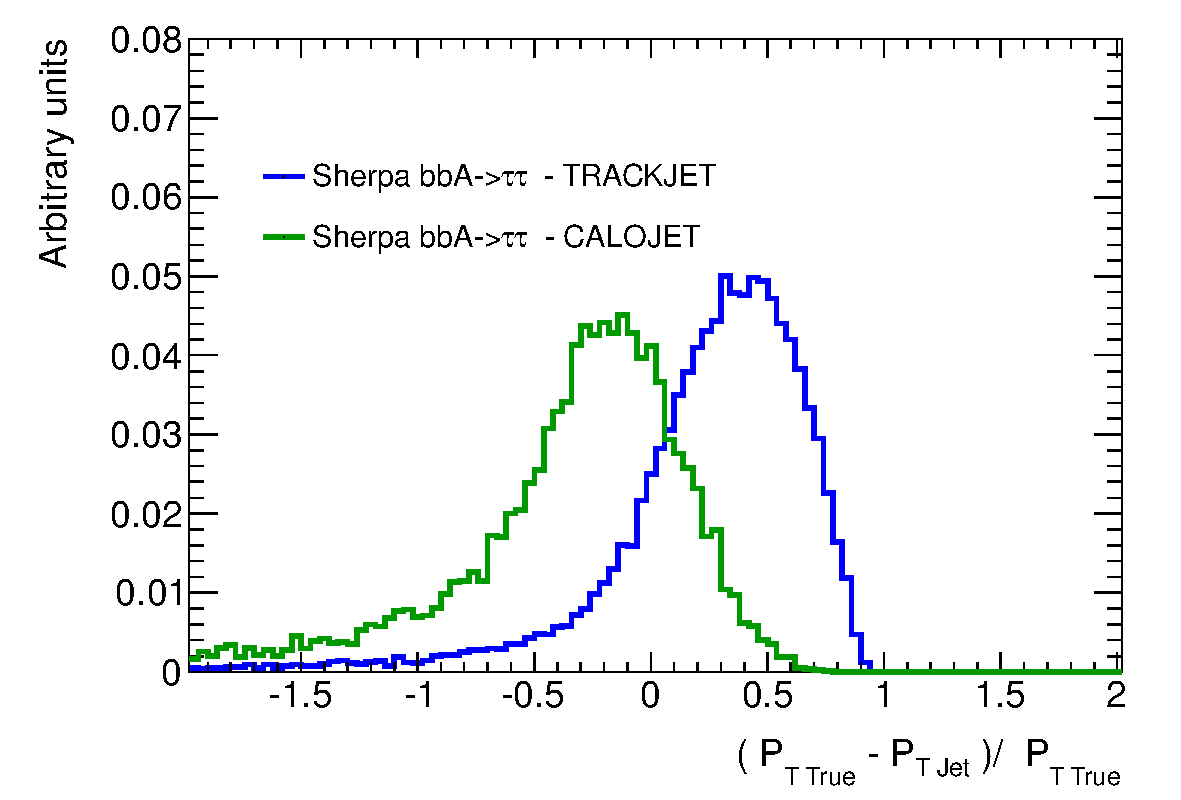
\includegraphics[width=0.6\textwidth]{figure/trackjet/residuals.pdf}
\caption{Residuals comparison of track-jet and calo-jet $\pt$ with respect simulated jet $\pt$.}
\label{fig:residuals}
\end{figure}    

To compare performance of track-jet and calo-jet, a cone size anti-kt 0.4 is choosen,
if a reconstructed jets lais up to a distance in $\Delta R $ < 0.3 from a simulated b-hadron
in the event, this jet is said to \emph{match with a b-hadron}. 
Reconstruction efficiency is then defined as the ratio between the number of matched b-hadron
and the total number of b-hadron. Figure~\ref{fig:recoEff} compare b-hadron reconstruction efficiency
between calo-jet and track-jets, the latter shows a higher reconstruction efficiency for low 
transverse momentum due to their robustness to pileup.
\begin{figure}[tp]
\centering
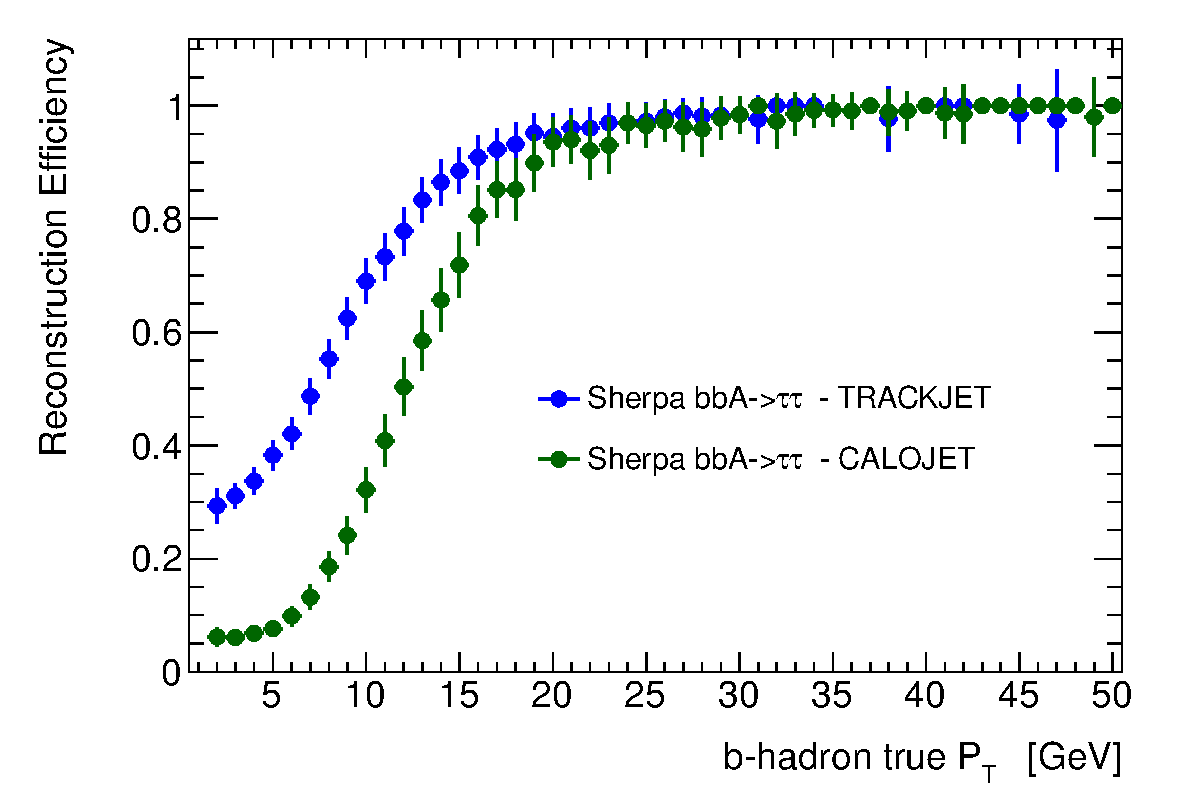
\includegraphics[width=0.6\textwidth]{figure/trackjet/recoEfficiency.pdf}
\caption{Comparison of b-hadron reconstruction efficiency for track-jet and calo-jet as a 
function of the simulated b-hadron $\pt$. Note that calo-jet and track-jet has a requirement 
at production level to be respectively with $\pt > 7$ and 2 GeV, a fair comparison is only possible
above 8 GeV in $\pt$.}
\label{fig:recoEff}
\end{figure}    

To exploit the performance of b-tagging on trackjets other two definitions are usefull: the tagging
efficiency and the rejection power. The \emph{tagging efficiency} is the fraction of \emph{matched} jets 
wich passes a determined selection on a tagging algorithm, i.e. which are \emph{tagged}.
The rejection is the inverse of the misidentifying rate, i.e. the inverse of the fraction 
of the jets which are not matched with a b-hadron or c-hadron, but are tagged. Fixing the selection
value for a given tagging algorithm will fix a point in the efficiency-rejection plane, this
is a common way in ATLAS to determine the performance of b-tagging and is shown in figure~\ref{fig:eff_rej},
figure~\ref{fig:rej_pt} instead shows the rejection as a function of the $\pt$ of the trackjet for the
tagging point which gives 50\% efficiency for that $\pt$ value. Mistagging rate is rapidly increasing
for low transverse momentum trackjets, revealing the necessity of a dedicated tagging algorithm for 
low $\pt$ jets.

\begin{figure}[tp]
\centering
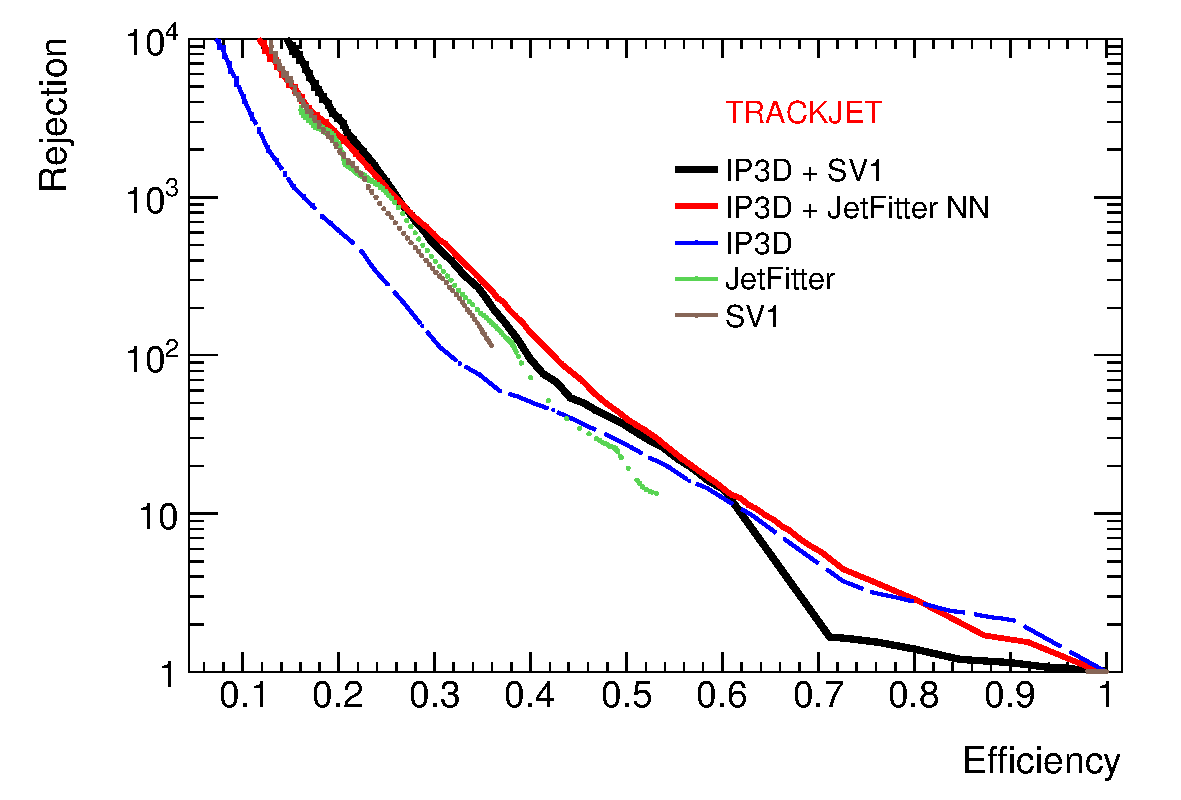
\includegraphics[width=0.7\textwidth]{figure/trackjet/std_eff_rej.pdf}
\caption{Rejection as a function of the tagging efficiency for different ATLAS tagging algorithm.}
\label{fig:eff_rej}
\end{figure}    

\begin{figure}[tp]
\centering
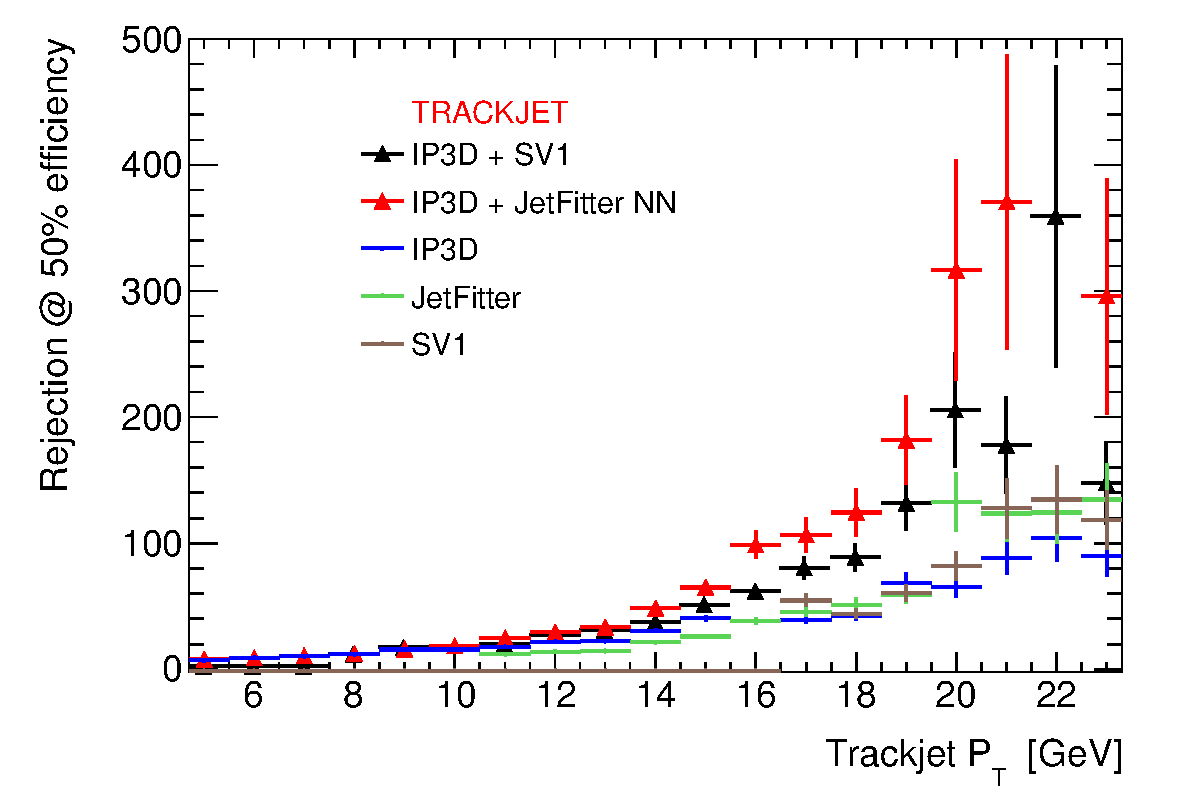
\includegraphics[width=0.7\textwidth]{figure/trackjet/std_rej_pt.pdf}
\caption{Rejection as a function of the transverse momentum of the trackjet for the
	tagging point which gives 50\% efficiency for that $\pt$ value. Different ATLAS tagging algorithm 
	are reported.}
\label{fig:rej_pt}
\end{figure}    

The previously introduced definitions do not allow a fair comparison between trackjets 
and calojets, due to the fact that calojets can be reconstructed also in case
no tracks are associated with them, in this particular case any tagging algorithm would likely fail,
altering the rejection distribution. It is convinient to use instead the following quantities,
\emph{effective rejection}, which is the inverse of the number of mistagged jets per event, and the
b-hadron \emph{reconstruction efficiency}, which is defined above. Figure~\ref{fig:cj_tj} shows 
a comparison between calojets and trackjets for the two variables just defined, for a given 
b-hadron reconstruction efficiency  trackjets can achieve higher rejection, for a fair 
comparison in this plot trackjets are selected in the transverse momentum range between 4 and 25 GeV, while
calojets between 8 and 50 GeV, this follow from figure~\ref{fig:residuals}. This demonstrates that 
thackjets are more suitable than calojets for low transverse momentum b-tagging.

\begin{figure}[tp]
\centering
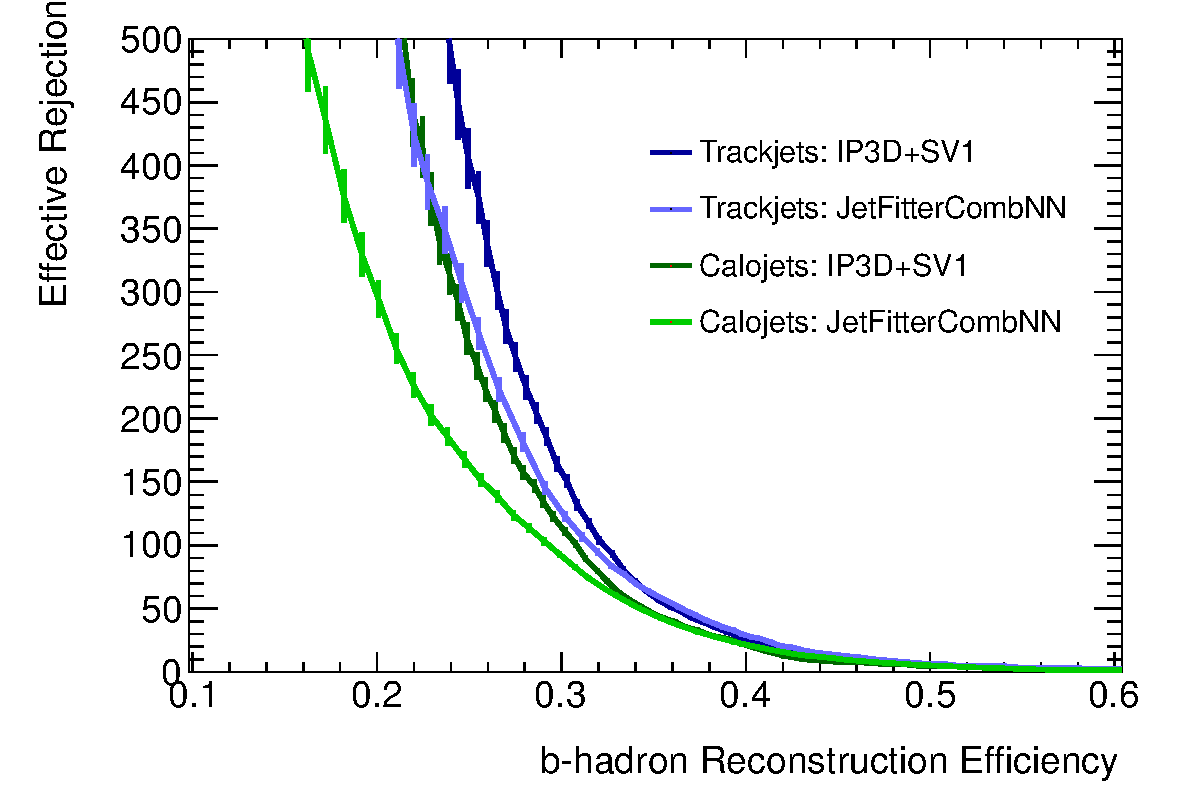
\includegraphics[width=0.7\textwidth]{figure/trackjet/eff_real_rej_mod.pdf}
\caption{Effective rejection as a function of b-hadron reconstruction efficiency, trackjet and calo jets are
	compared for two different ATLAS tagging algorithms. Trackjets are selected in the transverse momentum range 
	between 4 and 25 GeV, while calojets between 8 and 50 GeV.}
\label{fig:cj_tj}
\end{figure}    

%\subsection{Impact of Trackjet to the Analysis} % A new Hope
The impact of trackjets on the analysis is tested in a preliminary study, the yield of 
signal and for the most significant backgrounds is compared in table~\ref{tab:tj_cj},
where preselection is defined in a very similar\footnote{This study has not been updated 
with the newest version of the object reconstruction selections and corrections, a difference of the order of 10\%
is expected with respect the numbers in table~\ref{tab:eventsel:btag}.} 
way to what has been discuss in section~\ref{sec:topology} with the following exeption 
on the definition of taggable jets:
\begin{itemize}
\item Calorimeter taggable jets should have $|\eta| < 2.5$ and $20 < \pt < 50$ GeV
\item Track taggable jets should have $|\eta| < 2.5$ and $5 < \pt < 33$ GeV, this correspond to the same
  	range as for calojets above, figure~\ref{fig:residuals} in fact is only valid for low $\pt$ jets
	and the fraction of momentum lost approciate 1/3 for high $\pt$ trackjets. 
\end{itemize} 
As expected, given the higer reconstruction efficiency and the lower selection on $\pt$ of trackjets, they are
at b-taggin stage twice more efficient on signal and the request of a single b-jet is more efficient in reducing top background,
however, lower transverse momentum implies higer b-jet fake rates, which is seen in increasing $\Ztautau$ background, 
this may be a serious issue for QCD multi-jet background. The use of trackjets in the b-tag category is very promising
and can bring up to twice better sensitivity\footnote{Note that this estimate is done according to $s/\sqrt{b}$ ratio,
considering a counting experiment without systematic uncertainties and only two backgrounds, it represent then the upper limit 
to the gain in sensitivity with the current b-tagging performance.}, 
however to exploit the full power of this technique a dedicated b-tagging calibration on
trackjets is needed, furter study on improvement of low $\pt$ b-tagging are also auspicable, furthermore systematics uncertainty
on trackjets need to be evaluated, a preliminary study addressing one of the most important systematics for trackjets is 
reported in section~\ref{sec:trackjetsys}.
 
%\subsection{B-Discriminant} % variable to enhance low pT b-tagging
\begin{table}[tp]
	\begin{footnotesize}
	\begin{tabular}{p{3.0cm} |c c| c c| c c }
	\hline
	\hline\\ 
Selection 	& 	\multicolumn{2}{|c|}{Signal $bbA/H/h$ }	&\multicolumn{2}{c|}{$\Ztautau$}	& \multicolumn{2}{c}{$\ttbar$}	\\
	[0.5cm]
%	\noalign{\smallskip}
	\hline
Preselection		&	\multicolumn{2}{|c|}{$127.2 \pm 2.2$} &\multicolumn{2}{c|}{$3017 \pm 8$} &\multicolumn{2}{c}{$2066 \pm 5$} \\[0.5cm]
			&	Calojet		&	Trackjet &Calojet	&Trackjet	&Calojet	&Trackjet \\[0.5cm]
At least one taggable jet& $47.3 \pm0.8$	&$106.9 \pm1.8$	 &$1146 \pm3 $	&$2513 \pm 7$	&$1804 \pm 4$	&$2014 \pm 5$ \\[1cm]
Exactly one jet matched b-hadron& $18.4 \pm 0.3$ & $46.7 \pm 0.8$ & $4.5 \pm 0.3$	&$18.2 \pm 0.5$ 	&$1054 \pm 3$	&$959.1 \pm 2.3$  \\[1cm]
Exactly one tagged jet&	$10.2 \pm0.1$	&$21.0 \pm 0.6$	& $37.3 \pm 0.5$ &$107 \pm 1$ &$777 \pm 4$	&$630 \pm4$ \\[1cm]
	\hline
	\hline
	
	\end{tabular}
	\end{footnotesize}
	\caption{Impact of trackjets on the analysis, the event yield is compared between tracjets and calojets.
		For signal b-associated production is simulated for $\tan\beta=20$. The yields
		are normalized to an integrated luminosity of $1 ~ fb^{-1}$, all the selections are meant after preselection.}
	\label{tab:tj_cj}
\end{table}

\section{Systematic Uncertainties on Trackjets}\label{sec:trackjetsys}
\subsection{Introduction to Trackjet Systematics}
There are several sources that may give contribution to systematic uncertainties on the energy scale of trackjet, those
effects  are briefly summarized in what follows. Uncertainty can arise from MC generator details, like the particular 
choice of PDF and fragmentation fuction, details of the parton shower and underlying event, which in particular for low
transverse momentum object are known to be challenging to simulate, all those uncertainty can be evaluated by means of
a dedicated MC Rivet \cite{RIVET} analysis and will depend on the specific use of trackjets in the particular analysis,
the evaluation of this uncertainty, that will be different depending on the case, is then left to the analyzers of 
that analysis. Energy scale and resolution for single tracks is found to be very well modeled by simulation for tracks above
500 MeV \cite{IDperformance}, thus uncertainty on the energy scale and resolution that arise form mismodeling of
the pattern recognition algorithm are considered to be negligible. In dense track environment  different tracks may share 
same hits and this can genarate degradation of resolution, fake tracks, loss of track efficiency and in general can affect 
jet energy scale and resolution, this kind of effects has been checked in~\cite{JEStrack}, where calojet energy scale 
uncertainty are measured using tracks and has been shown that effects due to tracks hit merging are negligible 
for jets with $\pt < 300 $ GeV. Mismodeling of the inner detector material budged leads
to track reconstruction efficiency mismodeling, this strongly affects trackjets,
a methododology to estimate energy scale and recostruction efficiency uncertainty on trackjets due to material
budget mismodeling is presented for the first time in section~\ref{sec:trackExMat}.


\subsection{Material Budget Trackjets Uncertainty} \label{sec:trackExMat} %general description of the method
It can be shown that an increase or decrease of the material budged of the inner detector has as primary
effect the reduction or the increase of track reconstruction efficiency (see section~\ref{sec:valid}), 
for the estimation of the impact on a generic analysis that make use of trackjets would be rather uncenvinient 
to generate simulated sample with modified material budget, an easier approach would be then to
modify the track efficiency in a given sample according to its uncertainty~\cite{IDMaterial,trackEff}, and build 
out of trackjets out of the new collection of tracks, for a given sample however is only possible to reduce 
tracking efficiency, a tool has been build which generates out of the total tracks in the event a subsample
of tracks with inefficiency, trackjets which are build out of this subsample of tracks are called in the
following \emph{INEF-trackjets}. A minimum bias MC simulation sample is reproduced containing standard 
trackjets and INEF-trackjets, a set of "isolated" trackjet with cone size $\Delta R = 0.4$ are selected, meaning that no other trackjet 
should be reconstructed within a distance of $\Delta R = 0.8$. INEF-trackjets are then matched with the original trackjet
in an event by event basis via a cone matching, the matching fails if no INEF-trackjet is found within $\Delta R = 0.8$ from
the original one. Result on the deterioration of the trackjets efficiency and of the energy scale are presented respectively in 
figure~\ref{fig:inef_tj_std_eff} and~\ref{fig:inef_tj_std_scale}, based on the current knowledge of inner detector 
material budged~\cite{IDMaterial}, for low transverse momentum trackjets uncertainty on the material budget 
translates into an energy scale shift of 2-4\% and in a reduction of the mean number of tracks.
This method can only simulated effect of extra material (loosing track efficiency) but not of less material
(increased track efficiency), however, for the latter case a simmetric effect is expected.


\begin{figure}[tp]
\centering
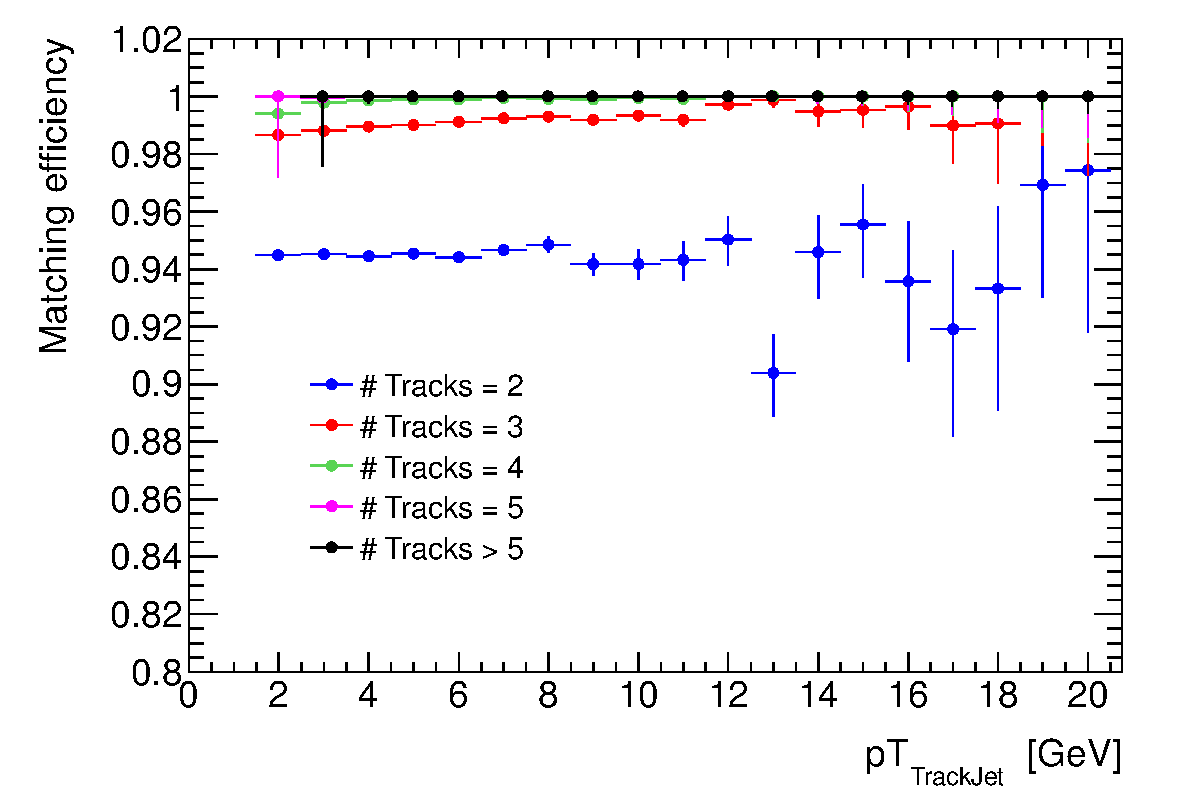
\includegraphics[width=0.7\textwidth]{figure/trackjet/T7/Sys_eff_n.pdf}
\caption{INEF-Trackjets are matched with standard trackjets, here is reported the matching efficiency as a function of 
	$\pt$ and number of track of standard trackjet.}

\label{fig:inef_tj_std_eff}
\end{figure}    

\begin{figure}[tp]
\centering
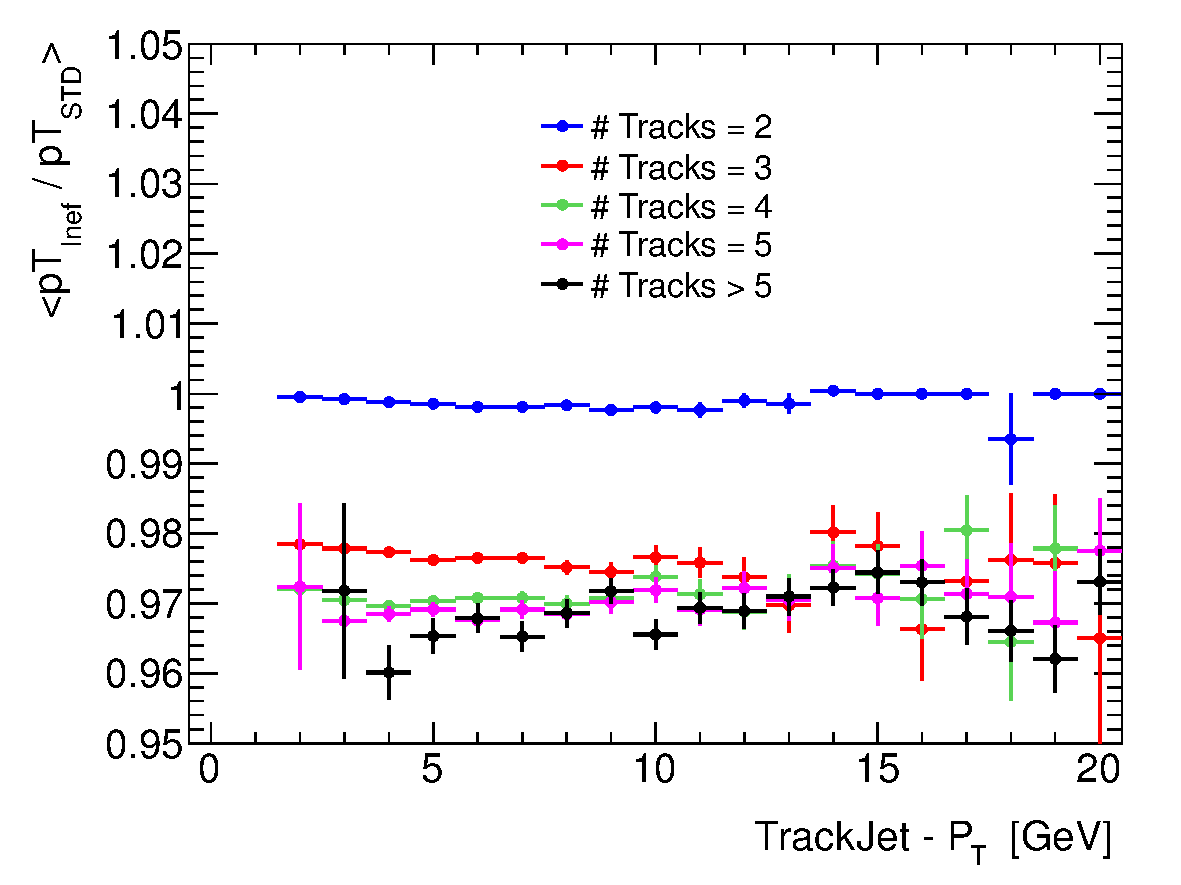
\includegraphics[width=0.7\textwidth]{figure/trackjet/T7/Sys_pt_nTrack.pdf}
\caption{INEF-Trackjets are matched with standard trackjets, here is reported the effect on the energy scale o
	as a function of $\pt$ and of the number of tracks of standard trackjet.} 

\label{fig:inef_tj_std_scale}
\end{figure}    


\subsection{Track Subtraction Validation} %confermo che l'effetto di Ex material e' solo efficiency
\label{sec:valid}
%effect on tracks of a 10% EX sample
The method described in section~\ref{sec:trackExMat} depends strongly on the assumption that the main effect of 
a modification of material budget is a loss or gain in track recontruction efficiency, i.e. that hadronic secondary
interaction in the inner detector leads manly to track lost and only in a marginal way in a decrease of track quality,
this is equivalent to say that the quality selection on tracks are robust enought.
In this section effect of budget material uncertainty on resolution and on the track fake rate are eveluated.
This is achieved by means of a MC simulation sample of minimum bias events where the effect of extra material is simulated
by increasing uniformly of 10\% the inner detector interaction lenght.  

Fake tracks are tracks that come from a random combination of hits generated from different particle, from simulation
is easy to identify this kind of "fake" by means of the truth particle to track matching, for simulated sample 
a particle to track match probability is stored, this correspond to the fraction of track hits for which that particle
is responsable, shared hits between more particles are weighted accordingly. The requirement on tracks are the ones defined 
in section~\ref{sec:tj_intro}, furthermore a track should be matched within $\Delta R <0.1$ with a 
stable\footnote{Here is intended a Generator stable and interacting particle, which means a charged particle with decay lenght > ,
also stable particle from secondary interactions are considered.} 
particle which has a matching probability with that track greather than 80\%. Tracks that do not fullfil
those requirements are called fakes. 
Resolution as shown in figure~\ref{fig:trk_reso} is about 1\% for large range of tracks $\pt$, difference in resolution between 
the extra material sample and the standard one can only introduce permill effect on the energy scale of a trackjet. 
The track fake rate, shown in figure~\ref{fig:trk_fakereate}, is also about 1-3\%, the extra material sample has 
a total increase of the track fake rate of permille. Figure~\ref{fig:trk_eff} shows the ratio of the track reconstruction
efficiency of primary particle between the standard and extra material sample, in the extra material sample is seen
a total decrease of the reconstruction efficiency of 1-2\%, loosing a track has a serious impact on trackjet energy scale.

\begin{figure}[tp]
\centering
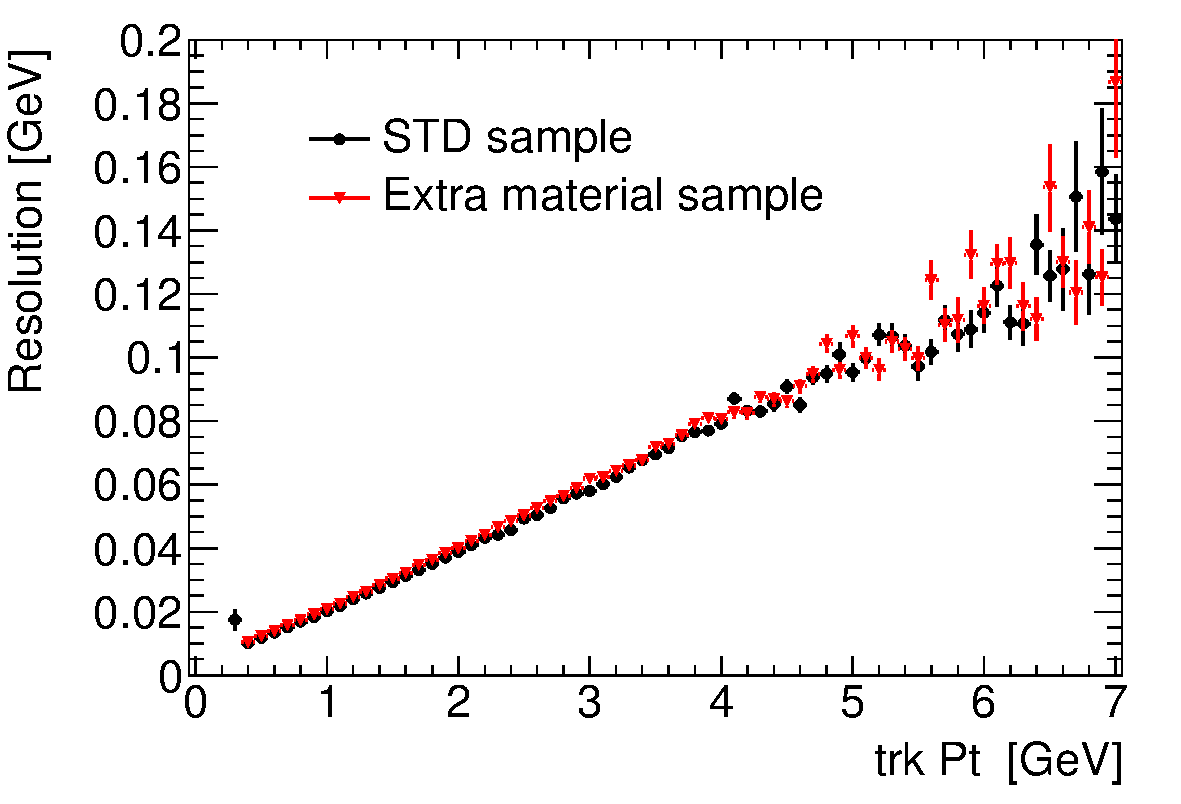
\includegraphics[width=0.45\textwidth]{figure/trackjet/T7/trk_reso_updater.pdf}
\caption{Track resolution with respect to matched truth particle as a function of truth particle $\pt$, 
	for standard Pythia minimum bias sample and 10\% inner detector extra material sample.}

\label{fig:trk_reso}
\end{figure}    

\begin{figure}[tp]
\centering
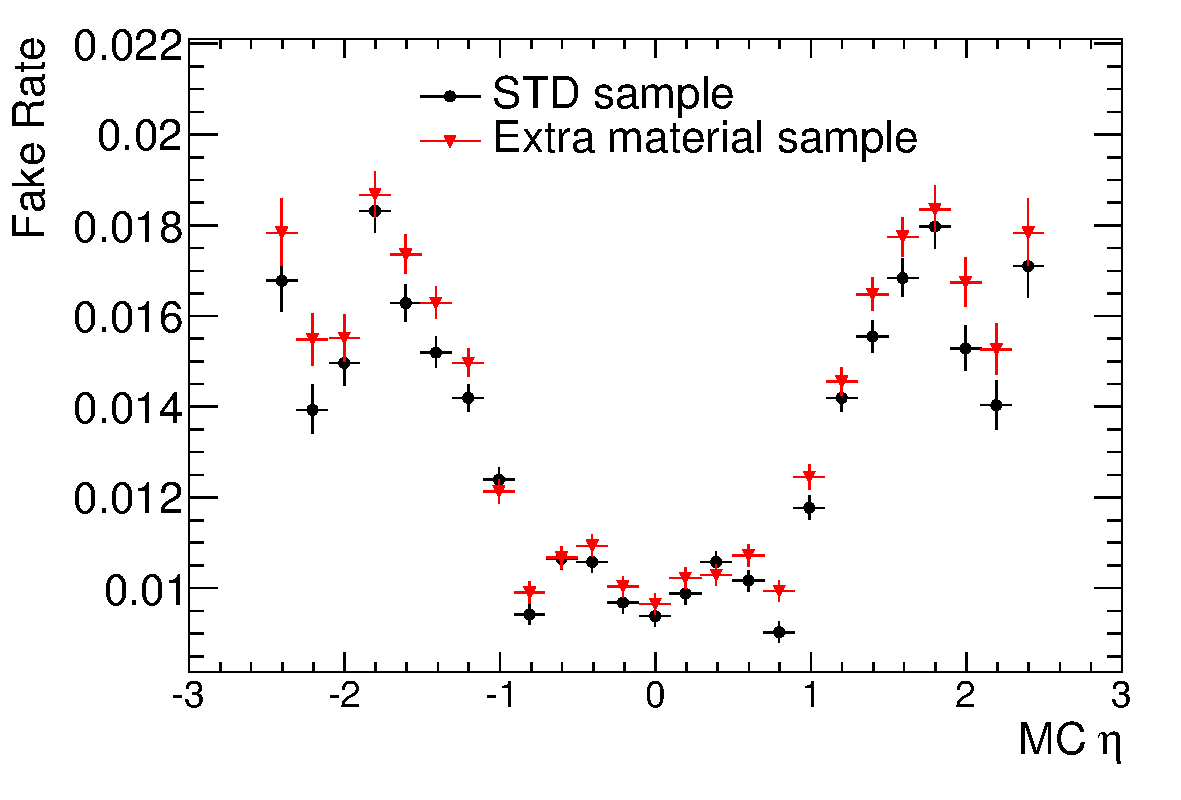
\includegraphics[width=0.45\textwidth]{figure/trackjet/T7/trk_fake_etauptade.pdf}
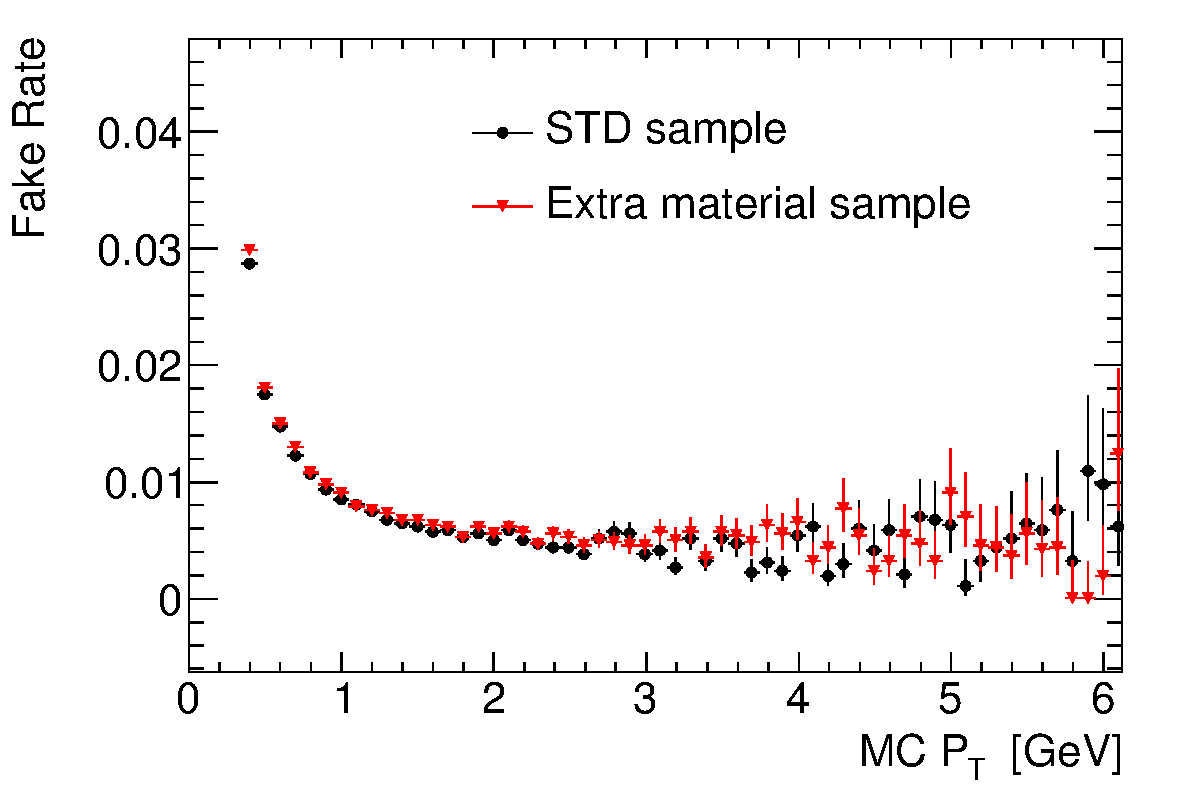
\includegraphics[width=0.45\textwidth]{figure/trackjet/T7/trk_fake_uptade.pdf}
\caption{Track fake rate resolution as a function of track $\eta$ (left) and track $\pt$ (right), for
	standard Pythia minimum bias sample and 10\% inner detector extra material sample.}

\label{fig:trk_fakereate}
\end{figure}    

\begin{figure}[tp]
\centering
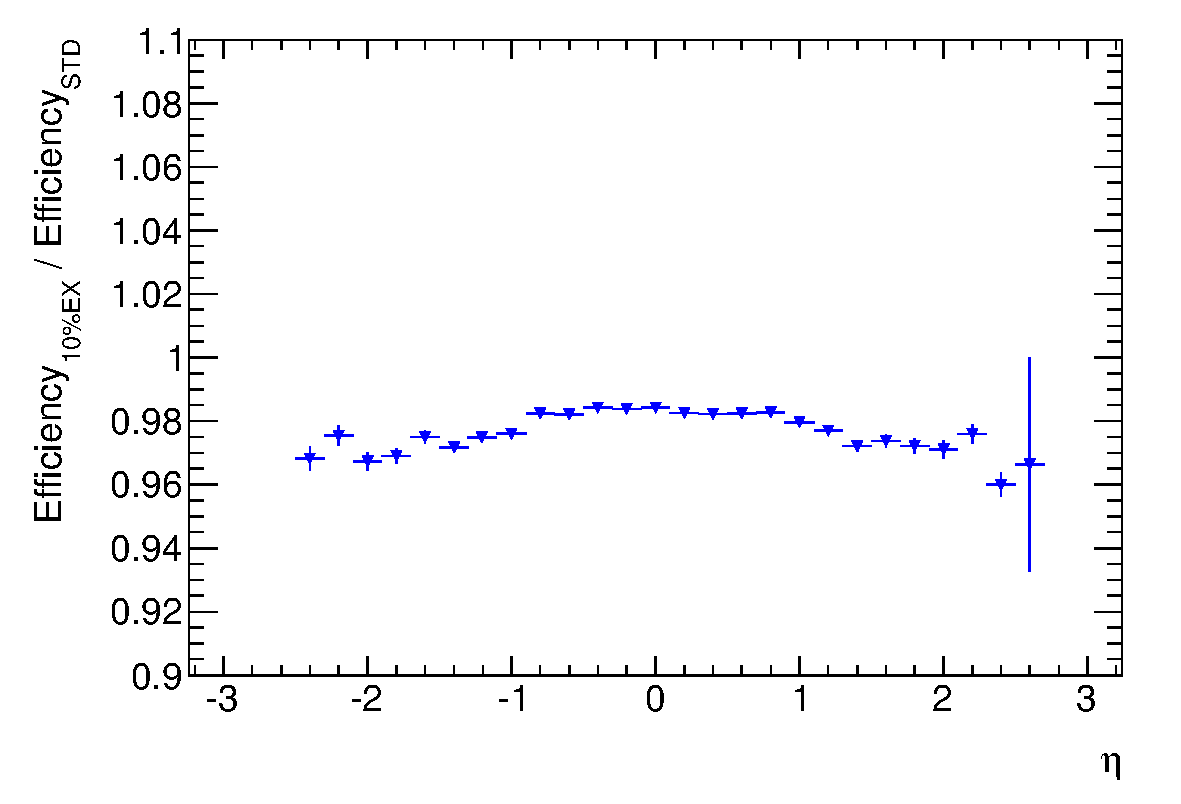
\includegraphics[width=0.45\textwidth]{figure/trackjet/T7/track_efficiency_ratio.pdf}
\caption{Track resolution efficiency with respect to primary truth particle as a function of truth particle $\eta$, 
	reported is the ratio between standard Pythia minimum bias sample and 10\% inner detector extra material sample.}

\label{fig:trk_eff}
\end{figure}    


Performance of INEF-trackjets (builded in a standard sample) are compared with the one of trackjets in the minimum bias extra material sample,
truth-jets (i.e. jets builded from truth particle) are matched with INEF-trackjets and trackjets respectively for comparison.



\begin{figure}[tp]
\centering
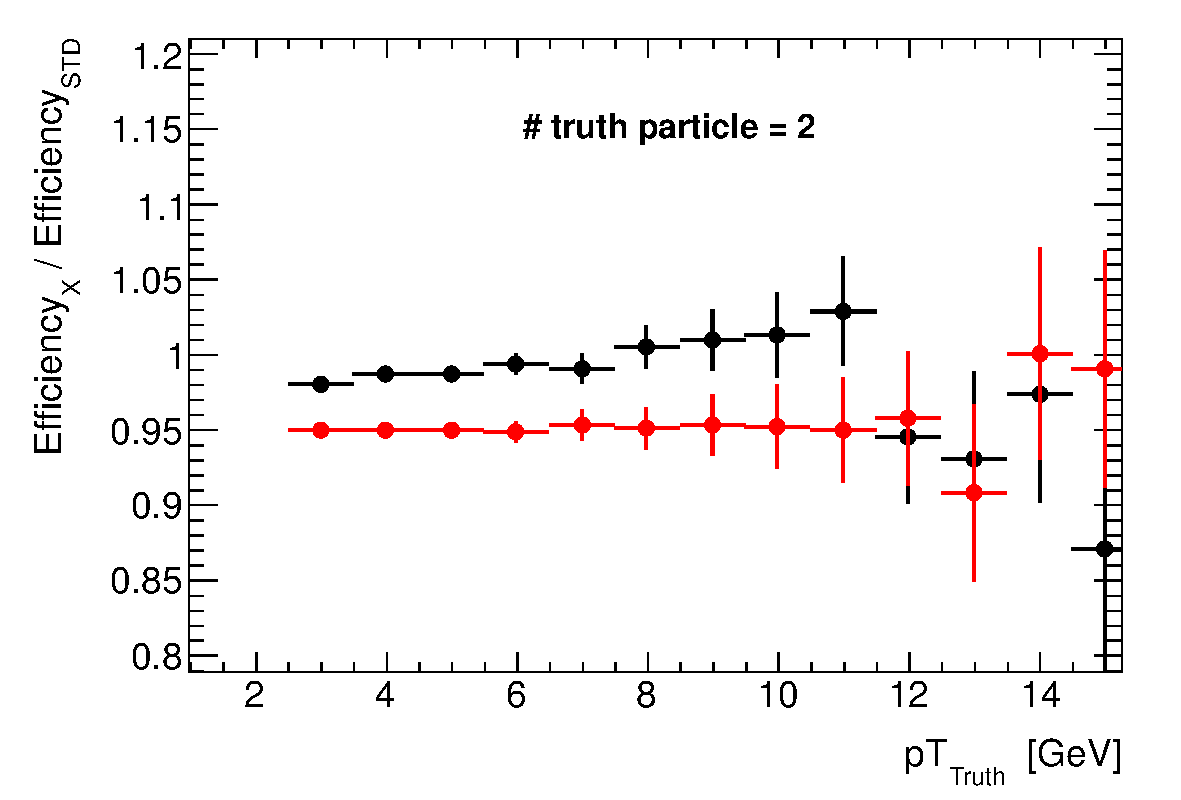
\includegraphics[width=0.45\textwidth]{figure/trackjet/T7/eff_ratio_2.pdf}
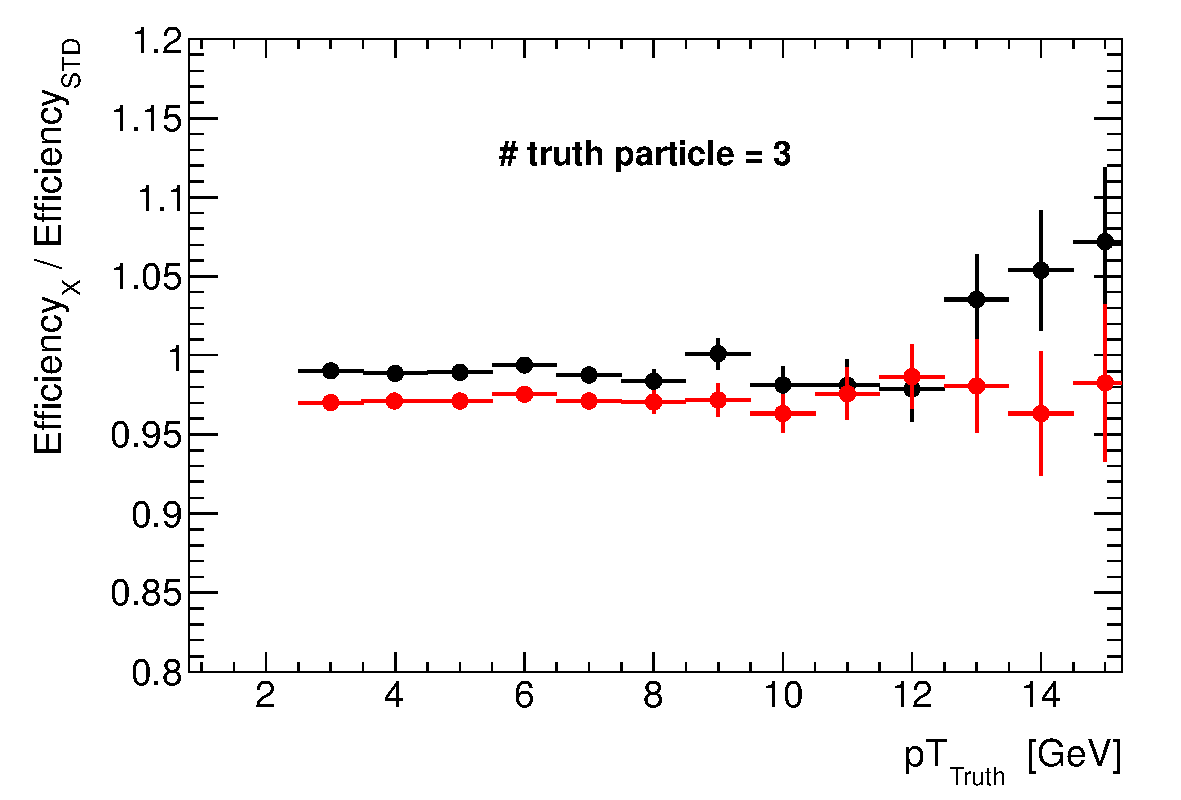
\includegraphics[width=0.45\textwidth]{figure/trackjet/T7/eff_ratio_3.pdf}
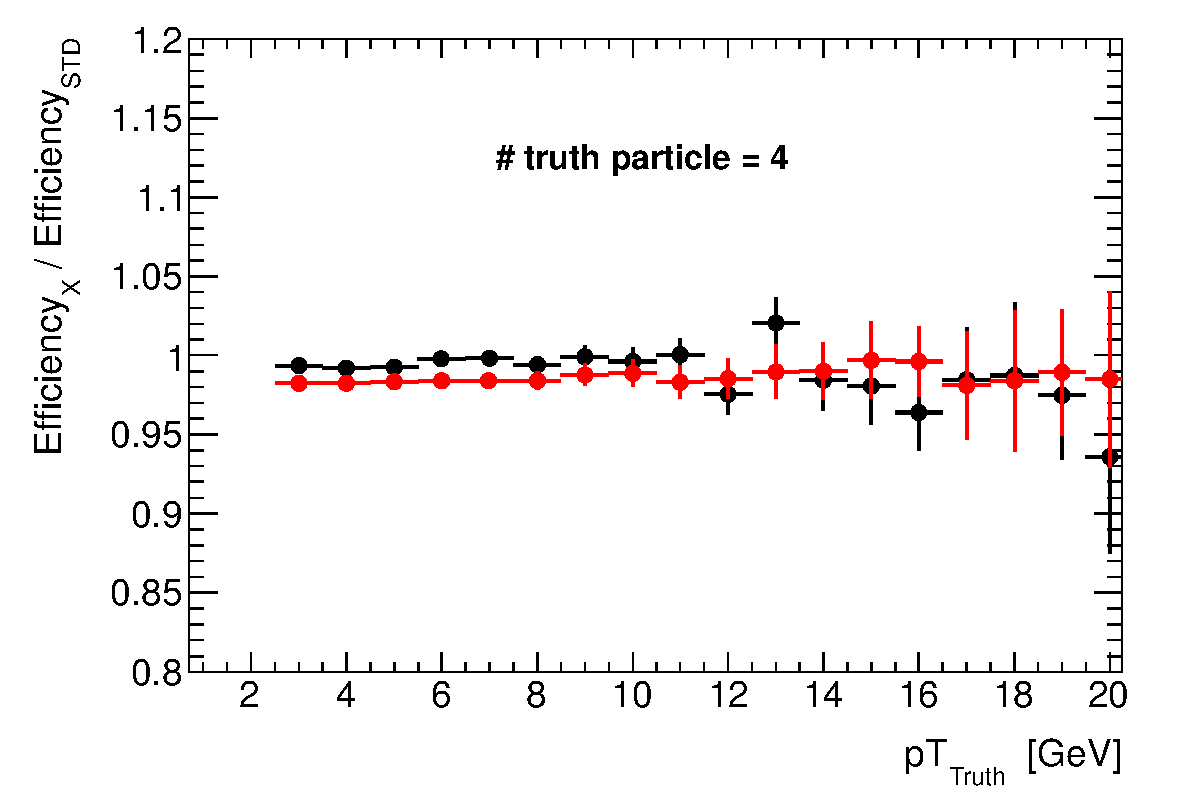
\includegraphics[width=0.45\textwidth]{figure/trackjet/T7/eff_ratio_4.pdf}
\caption{Ratio of efficiencies with respect to standard trackjets for INEF-trackjets and EX10-trackjets, in case of 2,3 and >4 track costituent.
	INEF-trackjets always reproduce correctly the inefficiency or give a conservative estimate.}

\label{fig:}
\end{figure}    

\begin{figure}[tp]
\centering
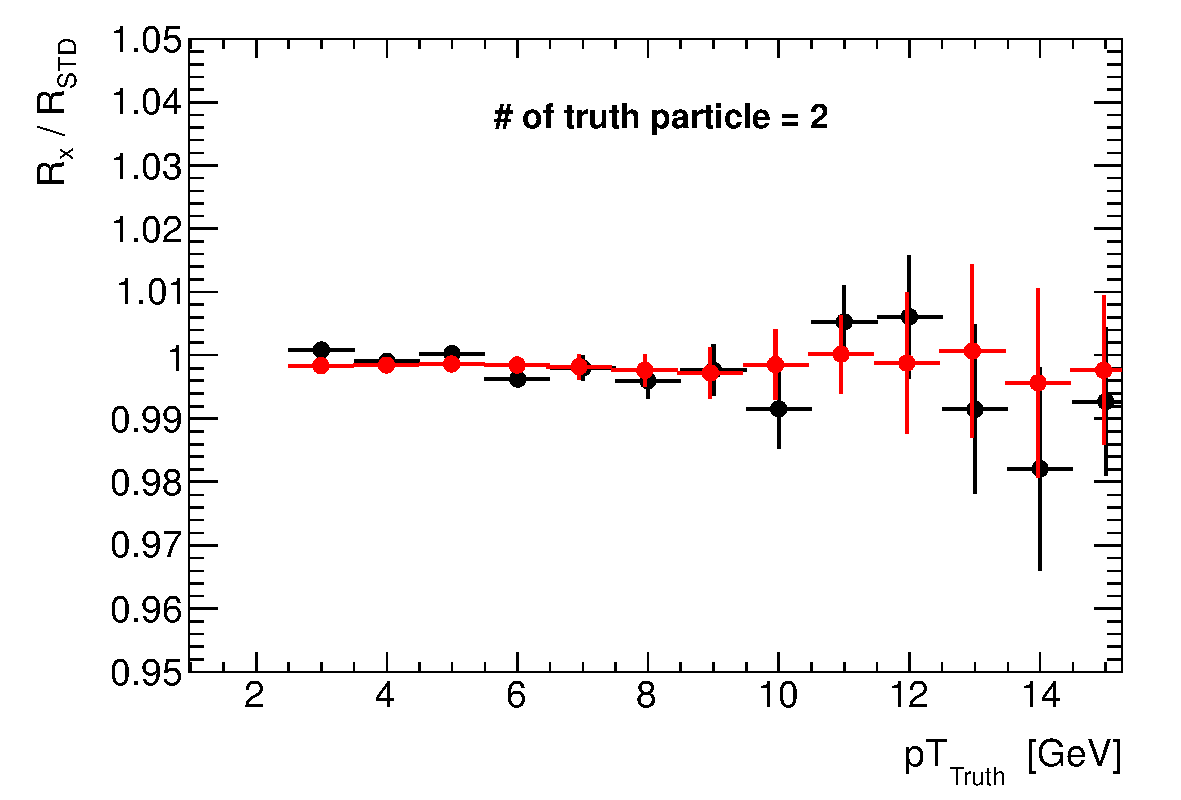
\includegraphics[width=0.45\textwidth]{figure/trackjet/T7/ratio_pt_2.pdf}
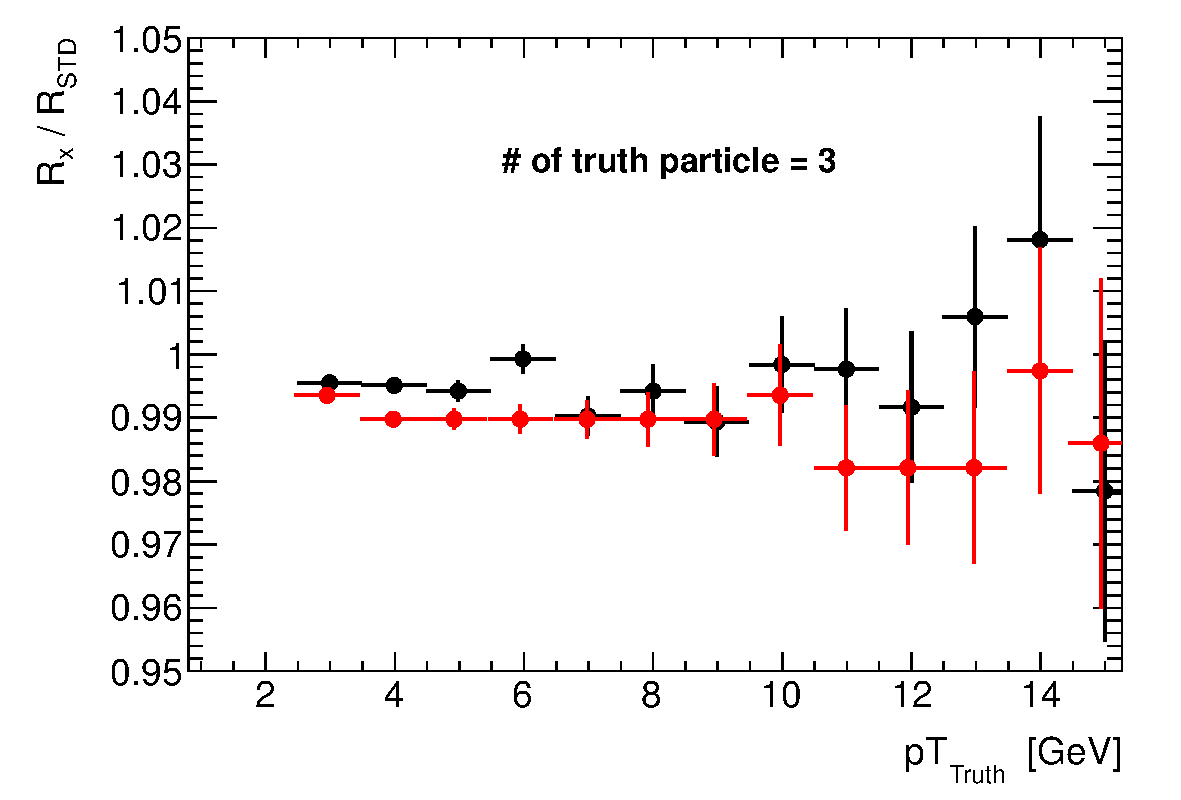
\includegraphics[width=0.45\textwidth]{figure/trackjet/T7/ratio_pt_3.pdf}
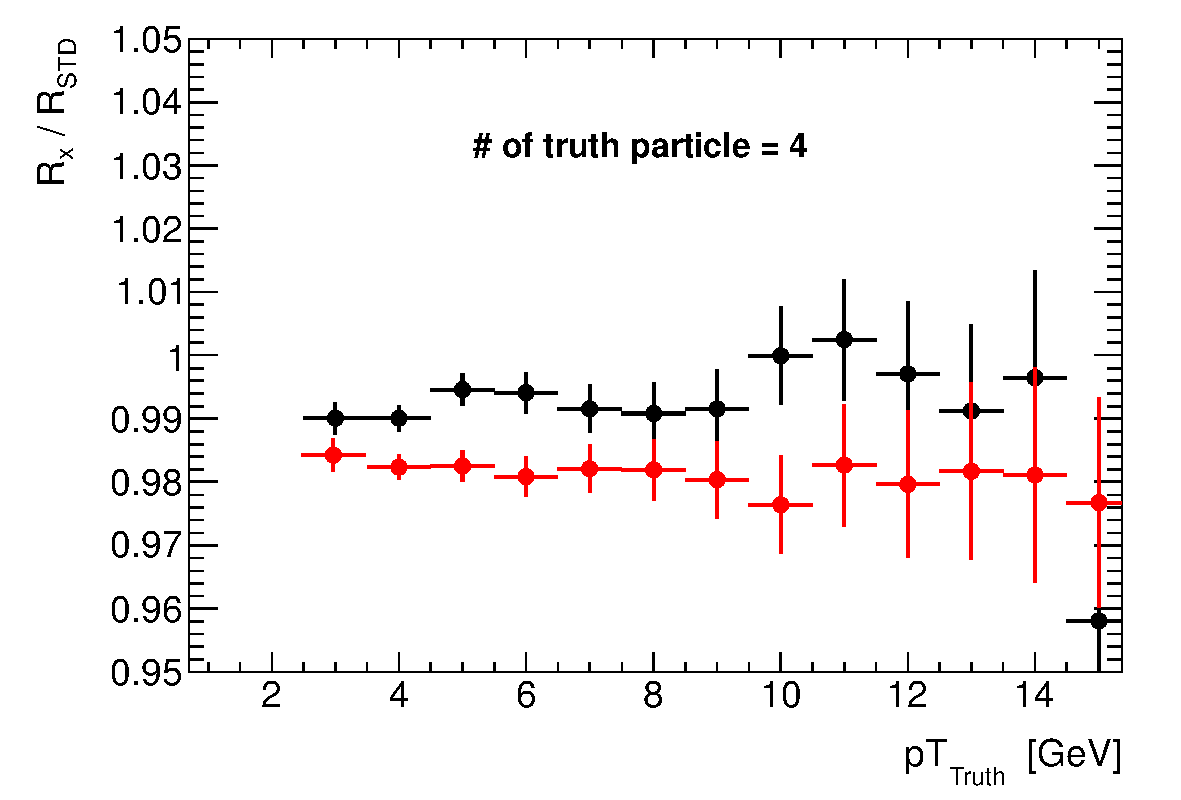
\includegraphics[width=0.45\textwidth]{figure/trackjet/T7/ratio_pt_4.pdf}
\caption{Ratio of energy scale with respect to standard trackjets for INEF-trackjets and EX10-trackjets, in case of 2,3 and >4 track costituent.
	INEF-trackjets always reproduce correctly the shift in energy scale or give a conservative estimate.}

\label{fig:}
\end{figure}    
























